\documentclass[a4paper,11pt]{article}
\pdfoutput=1 % if your are submitting a pdflatex (i.e. if you have
             % images in pdf, png or jpg format)

\usepackage{jcappub} % for details on the use of the package, please
                     % see the JCAP-author-manual

\usepackage[T1]{fontenc} % if needed
\usepackage{eucal}
\usepackage{xspace}
\usepackage{color}

\usepackage[justification=justified]{caption}


\title{ PyUltraLight: A Pseudo-Spectral Solver for Ultralight Dark Matter Dynamics}


%% %simple case: 2 authors, same institution
%% \author{A. Uthor}
%% \author{and A. Nother Author}
%% \affiliation{Institution,\\Address, Country}

% more complex case: 4 authors, 3 institutions, 2 footnotes
\author[]{Faber Edwards,}
\author[]{Emily Kendall,}
\author[]{Shaun Hotchkiss,}
\author[]{and Richard Easther}

% The "\note" macro will give a warning: "Ignoring empty anchor..."
% you can safely ignore it.

\affiliation[]{Department of Physics, University of Auckland, Private Bag 92019, Auckland, New Zealand}


% e-mail addresses: one for each author, in the same order as the authors
\emailAdd{faberedwards@gmail.com}
\emailAdd{eken000@aucklanduni.ac.nz}
\emailAdd{s.hotchkiss@auckland.ac.nz}
\emailAdd{r.easther@auckland.ac.nz}


\newcommand{\apj}{Astrophysical J.}
\newcommand{\prd}{Phys. Rev. D}
\newcommand{\mnras}{Mon. Notices Royal Astron. Soc}
\newcommand{\PyUltraLight}{\textsc{PyUltraLight}\xspace}
\newcommand{\re}[1]{\textcolor{blue}{[{\bf RE}: #1]}}

\abstract{\PyUltraLight  simulates the dynamics of ultralight dark matter in a static, non-expanding background.  \PyUltraLight can describe the evolution of several interacting ultralight dark matter halos  or one or more halos orbiting a central, fixed Newtonian potential, the latter scenario corresponding to dwarf galaxies orbiting a massive central galaxy. We verify  \PyUltraLight  by showing that it reproduces qualitative dynamical features of previously published simulations and demonstrate that it has  excellent energy-conservation properties.   \PyUltraLight is implemented in a Python-based Jupyter notebook, solving the Schr{\"o}dinger-Poisson equation  governing  ultralight scalar field dark matter dynamics in the non-relativistic regime using a symmetrised split-step pseudo-spectral  algorithm. The notebook interface makes it simple to specify simulation parameters and  visualise the resulting output. \PyUltraLight  runs on standard desktop hardware and is available on GitHub.  }




\begin{document}
\maketitle
\flushbottom

\section{Introduction}
\label{sec:intro}

The realisation that there may be more to the universe than meets the eye is one of the most profound developments in 20$^{\textrm{th}}$ Century astronomy and astrophysics. However,  while there are now multiple lines of evidence that dark matter outweighs baryonic matter by a ratio of approximately 5:1 \re{Add a citation to this}, we have few clues regarding the physical nature of dark matter.  Much theoretical and experimental effort has focussed on  WIMP models, motivated by their consistency with supersymmetric extensions to the Standard Model and their relatively simple dynamics. However but advanced direct-detection experiments are putting increasingly tight constraints on the WIMP parameter space \cite{Tan2016, Akerib2017} and $\Lambda$CDM cosmology with simple, pressureless, noninteracting dark matter (a class  including simple WIMP scenarios) is potentially at odds with observations at small astrophysical scales \cite{Bull2016}.  

The potential shortcoming of simple cold dark matter scenarios   motivate  investigations of more novel dark matter scenarios. In particular, ultralight dark matter (ULDM), also known as fuzzy dark matter (FDM), or BEC dark matter, is an increasingly well-studied possibility; for a recent review of the potential advantages and characteristic attributes of this scenario see Ref~\cite{Hui2016}.   ULDM models are well motivated by fundamental theories possessing approximate shift symmetries. Moreover, ULDM can naturally resolve the small-scale problems of $\Lambda$CDM as the Heisenberg uncertainty principle suppresses gravitational collapse on lengthscales shorter than the de Broglie wavelength of the ULDM particle. In this regime the mass of the ULDM particle becomes correlated with astrophysical observables; if it is on the order of $10^{-22}$~eV, structure is suppressed at kiloparsec scales and below \cite{Hu2000}. 


\re{read to here}The computational modelling of ULDM systems in the non-relativistic regime can be distilled into numerically solving the dynamical Schr{\"o}dinger-Poisson (SP) system of coupled differential equations for given initial conditions. Approaches to this problem have been varied, and have given rise to modifications of existing cosmological simulation codes as well as the development of new codes specifically for the modelling of ULDM systems, though public releases of the latter are  lacking. One approach has been to use the Madelung fluid formulation of the SP system \cite{Madelung1926}, in which there arises a quantum pressure term which can be treated numerically in a variety of ways. In \cite{Zhang2018}, the cosmological code \textsc{gadget} \cite{Springel2005} has been modified in order to treat this quantum pressure using an effective particle-particle interaction. This modified code, \textsc{axion-gadget}, has been made publicly available \cite{axion-gadget}. In \cite{Nori2018}, a non-public extension of \textsc{gadget}, \textsc{p-gadget3}, has been modified to treat the quantum pressure term using smoothed-particle hydrodynamics (SPH) routines. The SPH approach has also been used in \cite{Mocz2015}, while a particle-mesh approach was implemented in \cite{Veltmaat2016} to treat the quantum pressure term. Other cosmological simulation codes which have been recruited to solve ULDM dynamics (though not necessarily using the Madelung formulation) are N\textsc{yx} \cite{Almgren2013}, G\textsc{alacticus} \cite{Benson2012}, \textsc{arepo} \cite{Springel2010}, and \textsc{gamer} \cite{Schive2010, gamer}. N\textsc{yx} was modified in \cite{Schwabe2016} to study merging ULDM solitonic cores, G\textsc{alacticus} was modified in \cite{Du2017} to study the effects of tidal stripping and dynamical friction on ULDM halos, \textsc{arepo} was modified in \cite{Mocz2017} to study the core-mass relationship and turbulence characteristics of ULDM halos, and \textsc{gamer} was modified in \cite{Schive2014_b} to perform a detailed study of structure formation in ULDM cosmologies. 

While these modified cosmological simulation codes have produced promising results in the study of ULDM physics, at the time of writing only one such code, \textsc{axion-gadget}, has been made publicly available. The aim of this paper is to introduce \PyUltraLight, a stand-alone Python-based pseudo-spectral SP solver, and to demonstrate that this code is able to reproduce a number of key findings from the more complicated cosmological simulation codes without the need for high-performance computing environments. Consequently, we anticipate that as a publicly available resource, \PyUltraLight\ will serve as a valuable cross-check for more complex implementations and may serve as a basis for further development of such codes within the computational cosmology community.   

\PyUltraLight\ makes use of a symmetrised-split-step pseudo-spectral Fourier algorithm (also known as leap-frog) to compute the dynamics of the SP system. We note that a similar methodology has been described in \cite{Paredes2016}, though to the authors' knowledge this code has not been released publicly. The symmetrised-split-step method offers $2^{nd}$ order accurate time integration steps and sub-percent level energy conservation while normalisation of the wavefunction is conserved to machine precision. As a pseudo-spectral code, linear differential operators are computed by direct multiplication in the Fourier domain, while non-linear terms are evaluated in position space. This means that \PyUltraLight\ is free from noise associated with finite-differencing methods of computing spatial derivatives, though there is a necessary computational cost associated with the Fourier and inverse Fourier transforms. These transforms are optimised in \PyUltraLight\ through the use of the pyFFTW pythonic wrapper around the C-based FFWTW subroutine library \cite{pyfftw} \cite{fftw}. While the code is currently implemented to run on a singe machine, the FFTW libraries offer full parallelisation, so there is no barrier to running the code in a cluster environment.  

This paper is organised as follows. We first provide a short review of the physics of ULDM, including a derivation of the SP equations from an appropriate scalar-field Lagrangian. We then describe the details of the implementation of \PyUltraLight, before moving on to a testing and verification section, in which we reproduce a selection of results from a variety of recent ULDM simulations and discuss energy conservation within the code. 


\section{The Physics of ULDM}\label{sec:physics}

\subsection{The Schr{\"o}dinger-Poisson System}

The existence of an extremely light scalar field, minimally coupled to gravity, is the central premise on which ULDM models are predicated. Within the ULDM framework, it is proposed that large-scale cosmological structure formation proceeds through the Bose-Einstein condensation of this scalar field. In this section we derive the (non-relativistic) dynamical equations of the single macroscopic condensate wavefunction, namely, the Schr{\"o}dinger-Poisson equations. We begin by considering the following action functional for a scalar field, $\phi$, minimally coupled to gravity and in the absence of self-interactions:
\begin{equation}\label{eq:action}
    S=\int \frac{d^4x}{\hbar}\sqrt{-g}\bigg\{\frac{1}{2}g^{\mu\nu}\partial_\mu\phi\partial_\nu\phi-\frac{m^2}{2\hbar^2}\phi^2\bigg\},
\end{equation}
%
where we have taken $c=1$ but retain factors of $\hbar$ at this stage. Applying the variational principle to this action yields the Euler-Lagrange equations
%
\begin{equation}\label{eq:e-l}
    \frac{1}{\sqrt{-g}}\partial_\mu\big[\sqrt{-g}g^{\mu\nu}\partial_\nu\phi\big]-\frac{m^2}{\hbar^2}\phi=0.
\end{equation}
We evaluate equation \ref{eq:e-l} using linear perturbation theory, adopting the perturbed FRW metric in the Newtonian gauge:
\begin{equation}\label{eq:pFRW}
    ds^2=-\big(1+2\Phi(\vec{r})\big)dt^2+a(t)^2\big(1-2\Phi(\vec{r})\big)d\vec{r}^{\,2}.
\end{equation}
To linear order in $\Phi(\vec{r})$ we obtain 
\begin{equation}\label{eq:linear}
    \Ddot{\phi}-\frac{\big(1+4\Phi(\vec{r})\big)}{a(t)^2}\nabla^2\phi+3\big(1+2\Phi(\vec{r})\big)H\Dot{\phi}+\big(1+2\Phi(\vec{r})\big)\frac{m^2}{\hbar^2}\phi=0,
\end{equation}
where $H=\Dot{a}(t)/a(t)$. At late times, $H\ll m$ and it is sufficient to set $H=0$ and $a(t)=1$ in equation \ref{eq:linear}. In the non-relativistic limit, we may use the WKB approximation to obtain an ansatz solution to equation \ref{eq:linear}. We take 
\begin{equation}\label{eq:ansatz}
    \phi=\frac{\hbar}{\sqrt{2}m}\big(\psi e^{-imt/\hbar}+\psi^* e^{imt/\hbar}\big),
\end{equation}
where $\psi$ is a slowly varying complex function so that terms involving $\Ddot{\psi}$ may be neglected. We may also use $\nabla^2\phi\ll m^2/\hbar^2\phi$, such that our final result takes the form
\begin{equation}\label{eq:schrodinger}
    i\hbar\Dot{\psi}=-\frac{\hbar^2}{2m}\nabla^2\psi+m\Phi\psi.
\end{equation}
Thus, by making suitable approximations we have derived the Schr{\"o}dinger equation for $\psi$, which we now interpret as the unique macroscopic wavefunction of a Bose-Einstein condensate. It follows that the particle density of the condensate is given by $\vert\psi\vert^2$, such that the mass density is simply $m\vert\psi\vert^2$. Using this, we may therefore write down the Poisson equation as
\begin{equation}\label{eq:poisson}
    \nabla^2\Phi=4\pi G m \vert\psi\vert^2,
\end{equation}
where $G$ is Newton's gravitational constant. The coupled equations \ref{eq:schrodinger} and \ref{eq:poisson} together form the nonlinear Schr{\"o}dinger-Poisson (SP) system which describes the dynamics of ULDM in the non-relativistic regime. It is this system of equations which \PyUltraLight is designed to solve.


\subsection{Field Rescalings}

It is helpful to recast the SP system (equations \ref{eq:schrodinger} and \ref{eq:poisson}) in terms of adimensional quantities. In keeping with \cite{Schive2014} and \cite{Paredes2016}, we introduce length, time, and mass scales as follows:
\begin{align}
    \CMcal{L}&=\left(\frac{8\pi\hbar^2}{3 m^2H_0^2\Omega_{m_0}}\right)^{\frac{1}{4}}\approx121\left(\frac{10^{-23}\operatorname{eV}}{m}\right)\operatorname{kpc},\label{eq:length}\\
    \CMcal{T}&=\left(\frac{8\pi}{3 H_0^2\Omega_{m_0}}\right)^{\frac{1}{2}}\approx75.5 \operatorname{Gyr},\label{eq:time}\\
    \CMcal{M}&=\frac{1}{G}\left(\frac{8\pi}{3 H_0^2\Omega_{m_0}}\right)^{-\frac{1}{4}}\left(\frac{\hbar}{m}\right)^{\frac{3}{2}}\approx 7\times 10^7\left(\frac{10^{-23}\operatorname{eV}}{m}\right)\operatorname{M}_{\odot},\label{eq:mass}
\end{align}
where $m$ is the mass of the ultralight scalar field, $H_0$ is the present-day Hubble parameter, $G$ is Newton's gravitational constant and $\Omega_{m_0}$ is the present-day matter fraction of the energy density of the universe. We now recast equations \ref{eq:schrodinger} and \ref{eq:poisson} in terms of the following dimensionless quantities:
\begin{equation}\label{eq:dimensionless}
    t'=\frac{t}{\CMcal{T}},\quad
    \vec{x}^{\,'}=\frac{\vec{x}}{\CMcal{L}},\quad
    \Phi'=\frac{m\CMcal{T}}{\hbar}\Phi,\quad
    \psi'=\CMcal{T}\sqrt{mG}\psi.
\end{equation}
Dropping the primes for notational convenience, we see that the coupled differential equations of the SP system are reduced to 
\begin{align}
    i\Dot{\psi}(\vec{x},t)&=-\frac{1}{2}\nabla^2\psi(\vec{x},t)+\Phi(\vec{x},t)\psi(\vec{x},t),\label{eq:s-adim}\\
    \nabla^2\Phi(\vec{x},t)&=4\pi\vert\psi(\vec{x},t)\vert^2,\label{eq:p-adim}
\end{align}
where it is understood that all quantities involved are dimensionless. We can recover any dimensionful quantities of interest through simple transformations using equations \ref{eq:length} to \ref{eq:mass}. For example, the integrated mass of the system, $M_{tot}$, is given by
\begin{equation}\label{eq:integrated-mass}
    M_{tot}=\CMcal{M}\int d^3x\vert\psi\vert^2.
\end{equation}
Likewise, the mass density at any point is given by
\begin{equation}\label{eq:density}
    \rho=\frac{\CMcal{M}}{\CMcal{L}^3}\vert\psi\vert^2.
\end{equation}
All computations performed by \PyUltraLight\ are carried out using the dimensionless quantities defined in \ref{eq:dimensionless}, while provisions are made within the code for initial conditions and outputs to be converted to and from the desired unit system specified by the user. Henceforth, we will often refer to the quantity $\vert\psi\vert^2$ simply as the density, where it is understood that this is in fact a dimensionless quantity related to the physical mass density through a constant of proportionality given by equation \ref{eq:density}.




\section{Algorithm and Implementation}\label{sec:implementation}

In this section we discuss the methodology used to calculate the dynamics of the adimensional SP system (equations \ref{eq:s-adim} and \ref{eq:p-adim}) given user-specified initial conditions. We introduce the symmetrised split-step Fourier method, and describe schematically how the system is evolved at each timestep. 

\subsection{Dynamical Evolution}\label{sec:dynamics}

Dynamical evolution within \PyUltraLight\ progresses via a symmetrised split-step Fourier process on an $N\times N\times N$ simulation grid with spatial periodic boundary conditions. To understand this method, we first consider the exact expression for the unitary time evolution of the wavefunction according to equation \ref{eq:s-adim}, namely
\begin{equation}\label{eq:exact-time-ev}
    \psi(\vec{x},t+h)=\mathcal{T}\operatorname{exp}\left[-i\int_t^{t+h}dt'\left\{-\frac{1}{2}\nabla^2+\Phi(\vec{x},t')\right\}\right]\psi(\vec{x},t),
\end{equation}
where $\mathcal{T}$ is the time-ordering symbol. For sufficiently small timestep $h$, we can use the trapezoidal rule make the approximation
\begin{equation}
    \int_t^{t+h}dt'\Phi(\vec{x},t')\approx \frac{h}{2}\Big(\Phi(\vec{x},t\hspace*{-.2em}+\hspace*{-.2em}h)+\Phi(\vec{x},t)\Big).
\end{equation}
We can therefore write the approximate form of equation \ref{eq:exact-time-ev} as
\begin{equation}\label{eq:approx-time-ev}
    \psi(\vec{x},t+h)\approx \operatorname{exp}\left[i\frac{h}{2}\Big(\nabla^2-\Phi(\vec{x},t\hspace*{-.2em}+\hspace*{-.2em}h)-\Phi(\vec{x},t)\Big)\right]\psi(\vec{x},t).
\end{equation}
It is acknowledged that the exponential in equation \ref{eq:approx-time-ev} omits the time-ordering symbol, and is only equivalent to its time-ordered counterpart to order $h^2$.

Given that the linear differential operator in equation \ref{eq:approx-time-ev} acts naturally in Fourier space, while the nonlinear potential term is simplest to evaluate in position space, we are motivated to split the exponential so as to separate these terms. This will then allow us to employ a pseudo-spectral algorithm to compute the time evolution. Such a splitting of the exponential is valid when the timestep $h$ is small, as the dispersive and nonlinear terms can be assumed to act independently. In this implementation, we split the exponential as follows:
\begin{equation}\label{eq:split-step}
    \psi(\vec{x},t\hspace*{-.2em}+\hspace*{-.2em}h)\approx\operatorname{exp}\left[-\frac{ih}{2}\Phi(\vec{x},t\hspace*{-.2em}+\hspace*{-.2em}h)\right]\operatorname{exp}\left[\frac{ih}{2}\nabla^2\right]\operatorname{exp}\left[-\frac{ih}{2}\Phi(\vec{x},t)\right]\psi(\vec{x},t).
\end{equation}
This splitting can be understood thusly: first, a half timestep is taken in which only the nonlinear potential operator acts, followed by a full timestep in the linear term. The potential field is then updated, and a final half timestep in the nonlinear term is performed. We may use the Baker-Campbell-Hausdorff formula to express the product of exponentials in equation \ref{eq:split-step} as a single exponential. Keeping only terms to order $h^2$ we find:
\begin{equation}\label{eq:BCH}
    \operatorname{exp}\left[i\frac{h}{2}\Big(\nabla^2-\Phi(\vec{x},t\hspace*{-.2em}+\hspace*{-.2em}h)-\Phi(\vec{x},t)\Big)+\frac{h^2}{8}\Big[\nabla^2,\Phi(\vec{x},t)\Big]-\frac{h^2}{8}\Big[\nabla^2,\Phi(\vec{x},t\hspace*{-.2em}+\hspace*{-.2em}h)\Big]\right].
\end{equation}
Making use of the fact that $\Phi(\vec{x},t+h)\approx\Phi(\vec{x},t)+h\Dot{\Phi}(\vec{x},t)$, we see that the commutators in equation \ref{eq:BCH} cancel at $\mathcal{O}(h^2)$, such that this expression is equivalent to \ref{eq:approx-time-ev}, with the dominant error term appearing at $\mathcal{O}(h^3)$. 

Evaluation of equation \ref{eq:split-step} within \PyUltraLight proceeds as follows:
Initially, the nonlinear term acts in position space for one half-timestep. The result is then Fourier transformed, and a full timestep is taken in which the differential operator is applied in the Fourier domain. The potential field is then updated in accordance with equation \ref{eq:p-adim}. An inverse Fourier transform is then performed, and a final half timestep is taken in which the updated nonlinear term acts in position space to give the new $\psi$ field configuration. This procedure is known as the symmetrised split-step Fourier method, and is used widely in fields such as nonlinear fiber optics \cite{Agrawal2013}. It can be represented schematically as follows:
\begin{equation}\label{eq:schematic-psi}
    \psi(\vec{x},t\hspace*{-.2em}+\hspace*{-.2em}h)=\operatorname{exp}\left[-\frac{ih}{2}\Phi(\vec{x},t\hspace*{-.2em}+\hspace*{-.2em}h)\right]\CMcal{F}^{-1} \operatorname{exp}\left[\frac{-ih}{2}k^2\right]\CMcal{F}\operatorname{exp}\left[-\frac{ih}{2}\Phi(\vec{x},t)\right]\psi(\vec{x},t),
\end{equation}
where the order of operations is read from right to left, $\CMcal{F}$ and $\CMcal{F}^{-1}$ represent the discrete Fourier transform and its inverse, and $k$ is the wavenumber in the Fourier domain. The potential field is updated following the inverse Fourier transform in equation \ref{eq:schematic-psi}, and this update procedure may be represented schematically as
\begin{equation}\label{eq:schematic-phi}
    \Phi(\vec{x},t\hspace*{-.2em}+\hspace*{-.2em}h)=\CMcal{F}^{-1}\left(-\frac{1}{k^2}\right)\CMcal{F}\ 4\pi\vert\psi(\vec{x},t_{i})\vert^2,
\end{equation}
where $\psi(\vec{x},t_{i})$ represents the field configuration at this intermediary point in the timestep. The final operation in equation \ref{eq:schematic-psi} changes only the phase of the $\psi$ field, and thus we could replace $\psi(\vec{x},t_{i})$ with $\psi(\vec{x},t\hspace*{-.2em}+\hspace*{-.2em}h)$ in equation \ref{eq:schematic-phi} with no change in meaning. 

In the \PyUltraLight implementation, we make use of an additional simplification of the symmetrised split-step Fourier method. Namely, consecutive half-steps in the nonlinear term may be combined into a single full step in each case such that when iterated, only the first and last operations involve half steps. This can be represented schematically as 
\begin{equation}
    \psi(t\hspace*{-.2em}+\hspace*{-.2em}nh)=\operatorname{exp}\left[+\frac{ih}{2}\Phi\right]\left(\prod^n\operatorname{exp}\left[-\frac{ih}{2}\Phi\right]\operatorname{exp}\left[\frac{ih}{2}\nabla^2\right]\right)\operatorname{exp}\left[-\frac{ih}{2}\Phi\right]\psi(t),
\end{equation}
where the $\Phi$ field is updated at each step in accordance with equation \ref{eq:schematic-phi} and attention is drawn to the sign difference between the first and last operators.

The discrete Fourier transform (DFT) and its inverse are handled within \PyUltraLight using pyFFTW. pyFFTW is a pythonic wrapper around the C-based FFTW subroutine library, and allows for efficient evaluation of both real and complex DFTs \cite{pyfftw} \cite{fftw} \cite{Frigo2005}.  Multithreading is supported by pyFFTW, and is implemented within \PyUltraLight by using the multiprocessing package to determine the number of online CPUs and feed this directly to the threads argument of the pyfftw.FFTW class. 

In addition to the use of pyFFTW, performance within \PyUltraLight is further improved through the use of the NumExpr package, which provides routines for the efficient manipulation of array objects within the simulation using a vector-based virtual machine \cite{numexpr}. 

\subsection{Initial Conditions: Soliton Profiles}\label{sec:soliton-profiles}

The initialisation procedure within \PyUltraLight can be easily augmented to accommodate the requirements of the user. In the current implementation, the initial field configuration is built by loading a NumPy array file encoding a solitonic solution to the Schr{\"o}dinger-Poisson system. Using this method, solitons may be placed at the desired locations within the simulation grid, with the corresponding mass, velocity, and phase parameters each specified by the user within the accompanying Jupyter notebook. 

The solitonic solution to the SP system is a natural choice of initial field configuration; these stable, localised objects are ubiquitous in ULDM models \cite{Marsh2015}. 

%In particular, it is proposed that ULDM halos exhibit Navarro-Frenk-White profiles at large radii, with solitonic cores at smaller radii. Because solitons have a constant central density, it is suggested that this offers a solution to the core-cusp problem of $\Lambda$CDM \cite{Marsh2015}. 

%Remove this section if we're going to talk about solitons merging to form NFW/soltion profiles, and compare to e.g. Schwabe.

In this section, we discuss the method used to generate the soliton profile. Following \cite{Paredes2016}, we begin by assuming a spherically symmetric solution to the SP system:
\begin{equation}
    \psi(\vec{x},t)\rightarrow e^{i\beta t} f(r), \quad \Phi(\vec{x},t)\rightarrow \varphi(r),
\end{equation}
where $r=\vert\vec{x}\vert$. Introducing $\tilde{\varphi}(r):=\varphi(r)+\beta$, equations \ref{eq:s-adim} and \ref{eq:p-adim} are reduced to
\begin{align}
    0 &= -\frac{1}{2}f^{\prime\prime}(r)-\frac{1}{r}f^\prime(r)+\tilde{\varphi}(r)f(r)\label{eq:s-spherical}\\
    0 &= \tilde{\varphi}^{\prime\prime}(r)+\frac{2}{r}\tilde{\varphi}^\prime(r)-4\pi f(r)^2\label{eq:p-spherical}
\end{align}
where primes denote derivatives with respect to $r$. To generate profiles for $\tilde{\varphi}(r)$ and $f(r)$ which satisfy these equations, we use a fourth-order Runge-Kutta algorithm, included as the auxiliary soliton\texttt{\_}solution.py program. We make the arbitrary choice $f(r=0)$=1, while the smoothness criterion demands that the first derivatives of $f(r)$ and $\tilde{\varphi}(r)$ vanish at the origin. We then search for solutions of $f(r)$ and $\varphi(r)$ which satisfy the boundary conditions $\operatorname{lim}(r\rightarrow\infty)\varphi(r)=0$ and $\operatorname{lim}(r\rightarrow\infty)f(r)=0$. To do this we use a shooting method, varying $\tilde{\varphi}(r=0)$ until we obtain a solution of $f(r)$ which approaches zero at the maximal specified radius, $r_m$. The value of $\beta$ is then calculated by assuming that $\varphi(r)$ goes as $-c/r$ at large radii, where $c$ is a constant. Under this assumption, we can write
\begin{equation}
    \tilde{\varphi}(r_m)=-\frac{c}{r_m}+\beta, \quad c=r_m^2\tilde{\varphi}^{\ \prime}(r_m).
\end{equation}
We thus obtain the full solution $\psi(\vec{x},t)=e^{i\beta t}f(r)$.
Having initially chosen $f(r=0)=1$, we may then generalise to $f(r=0)=\alpha$, where $\alpha$ is an arbitrary positive real number. It is easy to verify that if $e^{i\beta t}f(r)$ is a solution to the spherically symmetric SP system, then $g(r)$ is also a solution, where
\begin{equation}
    g(r)=e^{i\alpha\beta t}\alpha f(\sqrt{\alpha}\ r).
\end{equation}
Hence we obtain a family of spherically symmetric soliton solutions to the dimensionless SP system, for which the dimensionless soliton mass is proportional to $\sqrt{\alpha}$ and the full width at half maximum is proportional to $1/\sqrt{\alpha}$. Because the size of the soliton scales inversely with the mass, it is important to consider the maximum soliton mass which can be accurately modeled in a simulation with finite spatial resolution. 

While the Schr{\"o}dinger equation is not trivially form invariant under Galilean boosts, we can enforce Galilean covariance by augmenting the solutions through the addition of a velocity-dependent phase factor. Namely,
\begin{equation}\label{eq:covariant-solution}
    \psi(\vec{x},t)=\alpha f\big(\sqrt{\alpha}\vert\vec{x}-\vec{v}t\vert\big)e^{i\left(\alpha\beta t+\vec{v}\cdot\vec{x}-\frac{1}{2}\vert\vec{v}\vert^2t\right)}.
\end{equation}
To construct the initial field configuration within \PyUltraLight, the NumPy array encoding the radial profile $f(r)$ for the $f(r=0)=1$ case is loaded, where the spatial resolution of this profile must agree with the expected spatial resolution within the main code. Equation \ref{eq:covariant-solution} is then used to augment the configuration such that the soliton is furnished with the position, mass, and velocity specified by the user in the accompanying Jupyter notebook. The user may also add an additional constant phase factor if desired.

While the current implementation of \PyUltraLight is designed such that the initial field configuration is built from solitons, it may be simply modified to take in alternative field configurations in future.  

\subsection{Timestep Constraints}

When using finite-differencing methods to solve certain partial differential equations, the causality-preserving Courant-Friedrichs-Lewy (CFL) condition on the size of the simulation timestep is a necessary condition for convergence \cite{Ajaib2013}. As such, this condition is often appears in numerical analysis of ULDM physics governed by the SP system, an example being \cite{Schwabe2016}. However, because \PyUltraLight does not use the method of finite differences to compute spatial derivatives, but rather computes them exactly via explicit multiplication in the Fourier domain, the CFL condition in its usual formulation is not applicable to this code. 

In place of the CFL condition, the constraint on the timestep within \PyUltraLight is set based on the fluid interpretation of the SP system. In dimensionless code units we can write 
\begin{equation}
    \psi\equiv\sqrt{\rho}e^{i\theta}, \quad \vec{v}\equiv\boldsymbol{\nabla}\theta.
\end{equation}
From here we can define a `maximum velocity' for the simulation grid. This is the velocity at which the fluid appears to move backward, which occurs when the phase change between successive grid points exceeds $\pi$. The timestep is then constrained such that a fluid travelling at this maximum grid velocity will traverse a distance of one grid space per timestep.

This proves to be a highly restrictive constraint on the timestep, and can be relaxed significantly at the user's discretion for simulations in which the expected velocities within the system will not approach this maximum grid velocity. Convergence testing on a case-by-case basis is encouraged to determine the timestep constraint necessary for a given degree of accuracy. 


\section{Verification of ULDM Dynamics}\label{sec:test}

In this section we test the validity of \PyUltraLight as a numerical SP solver by reproducing a number of results from previous studies of ULDM dynamics. We are able to reproduce phenomena arising due to the wavelike nature of ULDM, namely interference effects and effective repulsive forces. Additionally, we study the evolution of the velocity field within a solitonic core orbiting within a Newtonian central potential, showing that in the absence of complete tidal disruption, the stable orbital configuration is one of an irrotational Riemann-S ellipsoid. Finally, we demonstrate sub-percent level energy conservation for a selection of dynamical scenarios.

\subsection{Interference Patterns During Soliton Collisions}\label{sec:interference}

Hierarchical structure formation within the ULDM framework proceeds through both gravitational overdensity collapse as well as through sequential binary mergers of solitonic cores to form individual virialised objects \cite{Schive2014}. It is therefore important that ULDM simulations are able to accurately reproduce the expected characteristics of binary soliton interactions. 

Soliton collisions can be classified into two categories depending on whether the total energy of the isolated binary system is positive or negative. In the case of positive energy, the solitons pass through each other, emerging largely undisturbed from their initial configurations following the interaction. During the collision, the wavefunctions describing the solitons are superposed, yielding distinctive interference patterns. In this section we demonstrate the ability of \PyUltraLight to reproduce the interference patterns predicted by theoretical models during binary collisions. 

Following \cite{Schwabe2016}, we consider the head-on collision of two solitions with mass ratio $\mu=2$ and high relative velocity. Using equation \ref{eq:covariant-solution}, we can write the total wavefunction of the binary system in terms of dimensionless quantities along the collision axis as
\begin{align}
    \psi(x,t)=& \ \alpha_1 f\big(\sqrt{\alpha_1}\vert x-x_1-v_1 t\vert\big)e^{i\left(\alpha_1\beta t+v_1(x-x_1)-\frac{1}{2}v_1^2 t+\delta\right)}\nonumber\\
    &+\alpha_2 f\big(\sqrt{\alpha_2}\vert x-x_2-v_2 t\vert\big)e^{i\left(\alpha_2\beta t+v_2(x-x_2)-\frac{1}{2}v_2^2 t\right)}
\end{align}
where $x_1$ and $x_2$ are the initial positions of the centres of the solitions, $v_1$ and $v_2$ are the velocities of the solitons, $\delta$ is a constant relative phase term, and $\alpha_1=1/4 \ \alpha_2$ parameterise the density profiles as discussed in section \ref{sec:soliton-profiles}. Because of the symmetry of the configuration, we take $v_1=-v_2$ and $x_1=-x_2$. We are interested in the density profile of the system at the time of maximal interference, where we expect the superposed wavefunction to possess pronounced features. Therefore, we choose the time at which the two components of the wavefunction are centred at the same location, such that $x_1+v_1t=-x_2-v_2t=0$. This corresponds to a time $t_{max}=\vert x_1/v_1\vert = \vert x_2/v_2\vert$. The dimensionless density is then given by
\begin{align}\label{eq:predicted-interference}
    \vert\psi(x,t_{max})\vert^2= \ \alpha_1^2\bigg[&f(\sqrt{\alpha_1}x)^2+16f(2\sqrt{\alpha_1}x)^2+\nonumber\\
    &8f(\sqrt{\alpha_1}x)f(2\sqrt{\alpha_1}x)\operatorname{cos}\left(-3\alpha_1\beta\left\vert\frac{x_1}{v_1}\right\vert+2v_1x+\delta \right)\bigg]
\end{align}
In Figure \ref{fig:interference}, we plot the dimensionless density profile at the time of maximal interference for two solitons with mass ratio $\mu=2$, and phase difference $\delta=0$. We see that the numerical result obtained using \PyUltraLight closely matches the theoretical prediction of equation \ref{eq:predicted-interference}. Small disparities between the numerical and theoretical profiles may be attributed to the effect of gravitational contraction not included in the theoretical prediction of equation \ref{eq:predicted-interference}, and to a small offset in the true time of maximal interference. Neglecting these small deviations, we can verify that the code is well suited to faithfully reproduce the wave interference effects of the ULDM model. 
\begin{figure}
  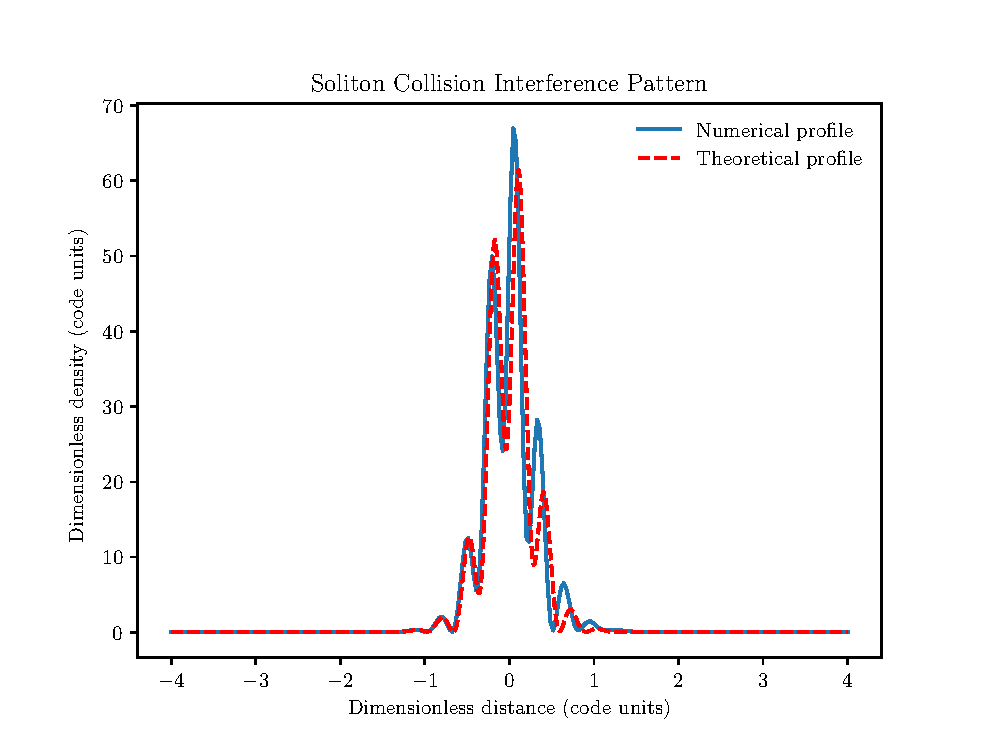
\includegraphics[trim={0 0 0 0.9cm},clip, scale=0.9]{interference_patterns}
  \caption{Comparison of theoretical and numerical density profiles at time of maximal interference for head-on collision of two solitons with mass ratio $\mu=2$ and no relative phase difference. The solitons were chosen with dimensionless masses 5 and 10, with an initial separation of 4 code units and relative velocity of 20 code units. The simulation was run at $256^3$ for a box of side-length 8 code units.}
  \label{fig:interference}
\end{figure}


\subsection{Effective Forces Due to Destructive Interference}

As demonstrated in \cite{Paredes2016}, the wavelike properties of ULDM can give rise to effective forces which can dramatically affect the dynamics of core collisions. These effective forces arise as a result of interference phenomena, and do not require the ULDM model to incorporate explicit local interactions. Figure \ref{fig:repulsion} shows the results of two simulations using \PyUltraLight in which two solitons of equal mass undergo a head-on collision. Contours of the density profile along the plane of symmetry are displayed. In the first simulation, there is no phase offset between the initial solitons, while in the second simulation the phases differ by $\pi$. We can see that the result of this phase shift is to create an effective repulsive force between the two solitons as they approach one another. Further discussion of this phenomenon and its possible observational consequences can be found in \cite{Paredes2016}.
\begin{figure}
  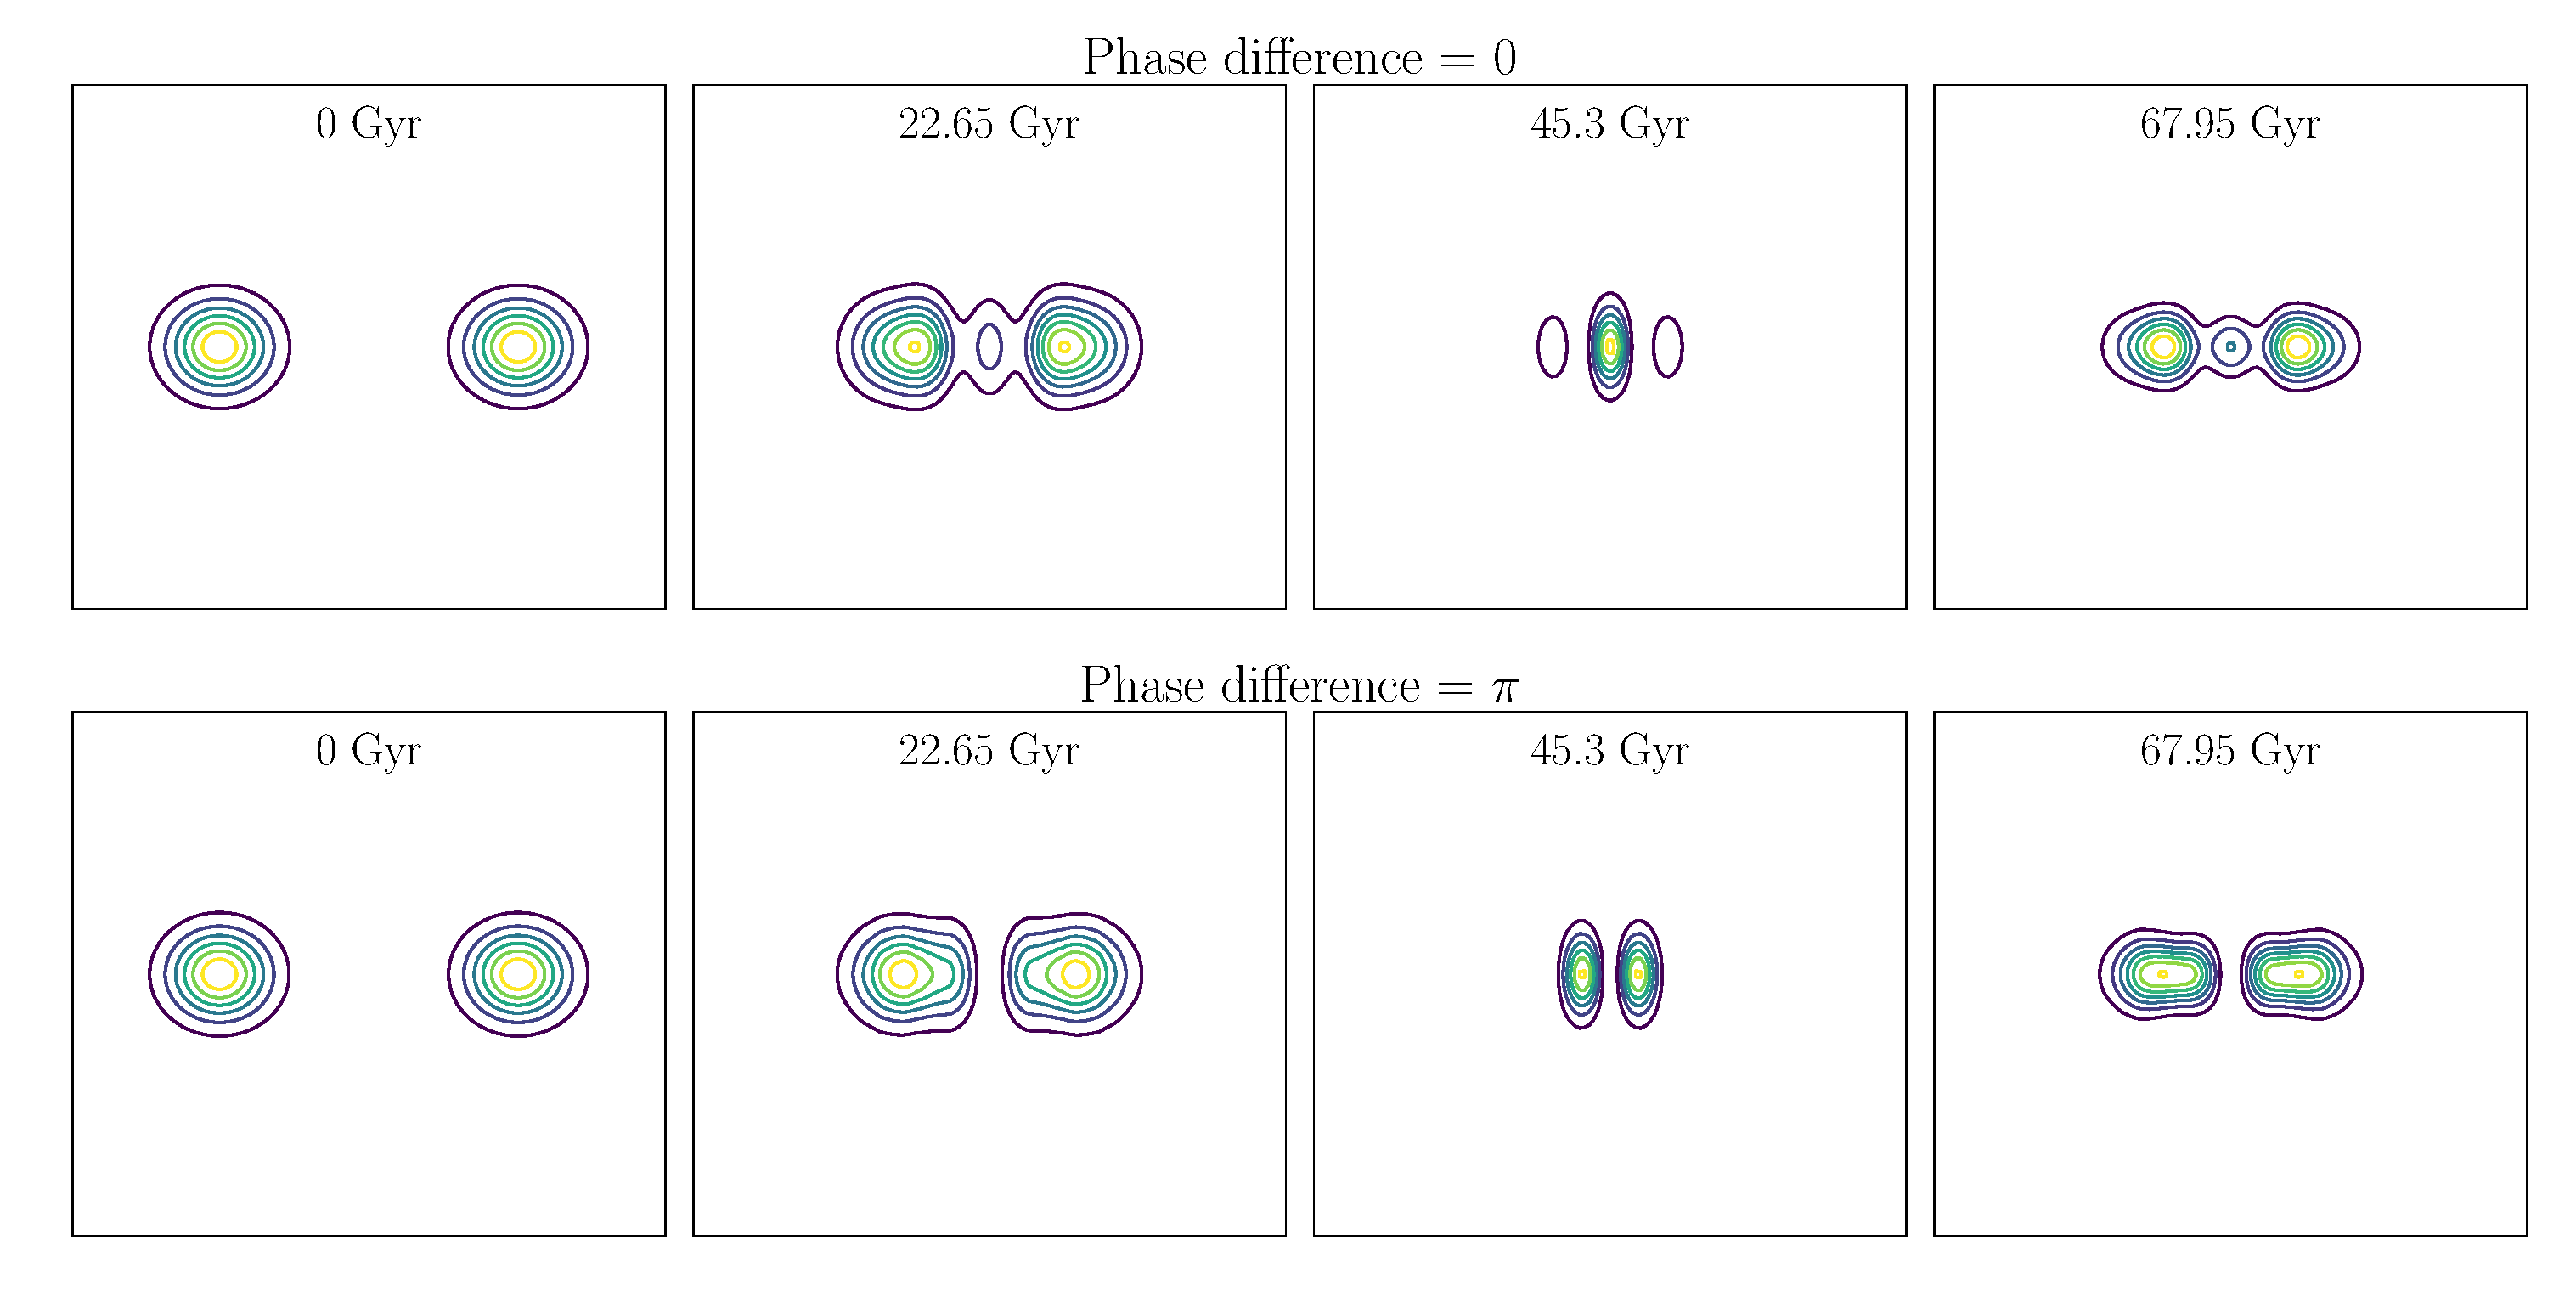
\includegraphics[width=1.\textwidth, trim={0 0 0 0},clip]{phase_comparison}
  \caption{Head-on collisions between two solitons of mass 5, relative velocity 6, and initial separation 4 in code units. Time progresses from left to right across each row.}
  \label{fig:repulsion}
\end{figure}

\vspace{1em}

\subsection{Tidal Disruption of Solitons Orbiting a Central Potential}\label{sec:disruption}

\PyUltraLight is designed such that a central potential may be included by way of a point-mass located at the centre of the simulation grid. While this setup is somewhat unphysical, it provides a starting point for a study of the stability of satellite dark matter halos orbiting a much larger object. Studies of this type can be used to make predictions regarding the lifespans of satellite galaxies around the Milky Way, offering a potential resolution of the so-called missing satellites problem \cite{Weinberg2015}.

An extensive study of the tidal disruption of ULDM solitonic cores orbiting a central potential has recently been undertaken in \cite{Du2018}. Here, we reproduce just one of their results as an additional validity check for \PyUltraLight. In particular, we reproduce the characteristic internal velocity field of a tidally-locked soliton orbiting a central potential. 

When the SP system is recast as a system of hydrodynamical equations, the fluid velocity is given by the gradient of the smoothly-varying phase at any point. This implies that the velocity flow of the SP system is irrotational, $\Nabla\times\vec{v}=0$. When a soliton is initialised in a circular orbit around a Newtonian potential, the initially spherical profile is distorted, elongated along the radial direction of the central potential. Meanwhile, the velocity field corresponding to the overall orbital motion of the soliton is superposed with the internal velocity field, combining so as to produce a net flow with vanishing curl. The family of Riemann-S ellipsoids describe uniformly rotating bodies which satisfy the condition of irrotationality \cite{Chandrasekhar1965}, and it is therefore the characteristic internal velocity field of such an ellipsoid which we expect to arise during the simulation. It is found in \cite{Du2018} that an initially spherical solitonic core without self-rotation will gradually spin up to form a tidally-locked irrotational Riemann-S ellipsoid when orbiting a host mass. We are able to reproduce this result using \PyUltraLight, with Figure \ref{fig:riemann} showing the internal velocity field of a solitonic satellite after one complete revolution around a host mass, obtained using \PyUltraLight on a $256^3$ simulation grid. In this case the ratio of host to satellite mass was $\approx 55$. It can be seen that the soliton has become elongated along the radial line connecting to the host, indicating that it is tidally locked. Meanwhile the internal velocity field can be seen to be that of an irrotational Riemann-S ellipsoid \cite{Daller2012}.
\begin{figure}
  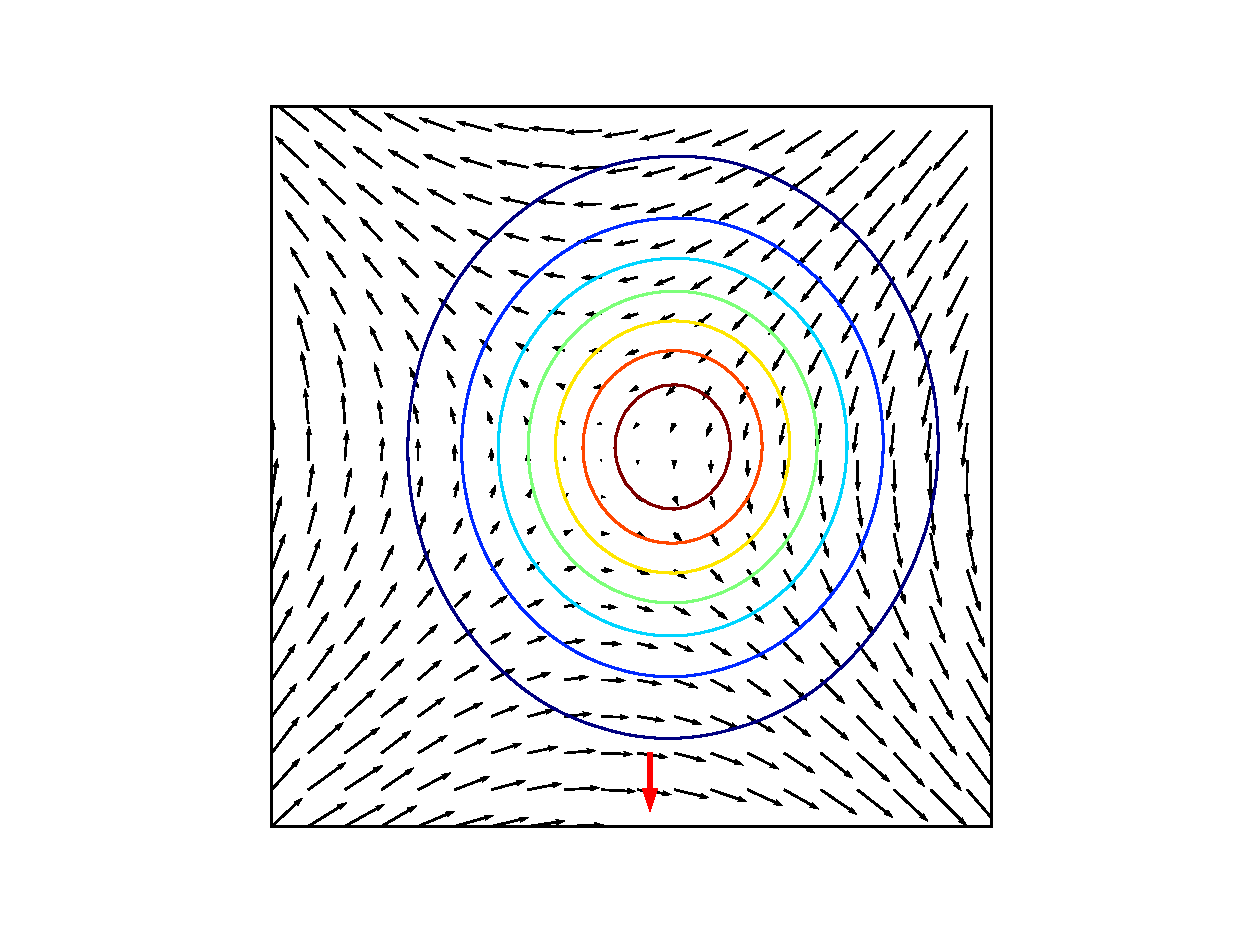
\includegraphics[width=1.\textwidth,trim=1cm 1cm 0 1cm,clip]{riemann}
  \caption{Solitonic core after one revolution of a central potential, demonstrating the internal velocity field of an irrotational Riemann-S ellipsoid (where the collective motion of the soliton has been subtracted from the velocity field). Deformation of the spherical density profile into that of an ellipsoid can be seen, with extension along the radial direction (red arrow).}
  \label{fig:riemann}
\end{figure}

\vspace{1em}

\subsection{Energy Conservation}\label{sec:energy}

In addition to the evolution of the condensate wavefunction $\psi$ and the potential $\Phi$, \PyUltraLight also evaluates the energy of the SP system. An important achievement of the code is sub-percent level energy conservation, even at relatively low spatial resolution, for all dynamical scenarios tested. In this section we derive the expression for the total energy of the SP system and discuss its decomposition into individual constituents calculated separately within the code. We then present the numerical energy evolution of a variety of configurations. 

We begin by defining a suitable action which yields the full SP system through its corresponding Euler-Lagrange equations. We find that variation of
\begin{equation}\label{eq:sp-action}
    S=\int dt\int_{\mathbb{R}^3} d^3x \  -\bigg\{\frac{1}{2}\vert\nabla\Phi\vert^2+\Phi\vert\psi\vert^2+\frac{1}{2}\vert\nabla\psi\vert^2+\frac{i}{2}(\psi\Dot{\psi}^*-\Dot{\psi}\psi^*)\bigg\}
\end{equation}
with respect to $\Phi$, $\psi^*$ and $\psi$ yields equations \ref{eq:p-adim}, \ref{eq:s-adim}, and the conjugate of equation \ref{eq:s-adim}, respectively. The integrand of equation \ref{eq:sp-action} is the Lagrangian density, $\mathcal{L}$, from which we can derive the conserved energy in the usual way:
\begin{equation}
    E_{tot}=\int_{\mathbb{R}^3}d^3x \ \bigg\{\frac{\partial \mathcal{L}}{\partial \Dot{\psi}}\Dot{\psi}+\frac{\partial \mathcal{L}}{\partial \Dot{\psi}^*}\Dot{\psi}^*+\frac{\partial \mathcal{L}}{\partial \Dot{\Phi}}\Dot{\Phi}-\mathcal{L}\bigg\}.
\end{equation}
Evaluating this expression, we obtain:
\begin{align}
    E_{tot}&=\int_{\mathbb{R}^3}d^3x \ \bigg\{\frac{1}{2}\vert\nabla\Phi\vert^2+\Phi\vert\psi\vert^2+\frac{1}{2}\vert\nabla\psi\vert^2\bigg\}\\
    &=\int_{\mathbb{R}^3}d^3x \ \bigg\{\frac{1}{2}\nabla(\Phi\nabla\Phi)-\frac{1}{2}\Phi\nabla^2\Phi+\Phi\vert\psi\vert^2+\frac{1}{2}\nabla(\psi^*\nabla\psi)-\frac{1}{2}\psi^*\nabla^2\psi\bigg\}\\
    &=\int_{\mathbb{R}^3}d^3x \ \bigg\{\frac{1}{2}\Phi\vert\psi\vert^2-\frac{1}{2}\psi^*\nabla^2\psi\bigg\}.\label{eq:energy-tot}
\end{align}
where in the last step we have used Stokes' Theorem as well as the Poisson equation (\ref{eq:p-adim}) to perform simplifications. Because we are working with the dimensionless quantities defined in equation \ref{eq:dimensionless}, it is easy to see that this quantity is related to the physical energy through multiplication by a constant factor of $\CMcal{L}^5\CMcal{T}^{-4}G^{-1}$. It should be noted that equation \ref{eq:energy-tot} is not equivalent to the expectation value of the Schr{\"o}dinger Hamiltonian, which is itself not a conserved quantity of the SP system and is given by
\begin{equation}
    \langle\hat{H}\rangle=\int_{\mathbb{R}^3}d^3x \ \bigg\{\Phi\vert\psi\vert^2-\frac{1}{2}\psi^*\nabla^2\psi\bigg\}.
\end{equation}

The two terms in the integral \ref{eq:energy-tot} are calculated separately within the code. It is easy to see that the first term represents the gravitational potential energy of the SP system. As discussed in \cite{Hui2016}, the second term may be decomposed further into two contributions which may be considered separately as kinetic and `quantum' energies, but for the purposes of this implementation it is sufficient to consider only their combined contribution. Because \PyUltraLight provides the option to include the central potential of a point mass located at the centre of the simulation grid, we have additional energy contributions when such a potential is included. Because this central potential does not arise from a ULDM object, we calculate the gravitational potential energy due to self-interaction separately from the gravitational potential energy due to the central potential.

Figures \ref{fig:combined_1} and \ref{fig:binary} demonstrate energy conservation for two example simulation scenarios. In the first case, we examine the evolution of the energy for a single soliton undergoing significant tidal disruption within a Newtonian central potential. We see that as the soliton is disrupted, the kinetic energy increases, while the gravitational energy due to the central potential decreases, as expected. Meanwhile, the gravitational potential energy due to self-interaction gradually increases toward zero as the disruption continues. The sum of the individual energy components is conserved to $10^{-2}\ \%$ in this case, where the simulation was run at $256^3$. Higher grid resolutions result in even better energy conservation. Figure \ref{fig:binary} demonstrates the evolution of the energy of a binary system of solitons in elliptical orbits around their common centre of mass. In this case the simulation ran for approximately three orbital periods at $256^3$. At points of closest approach, it can be clearly seen that the kinetic energy increases as the solitons speed up, while the potential energy due to self-interaction decreases commensurately. In this scenario no central potential has been included, so the gravitational energy due to the central potential stays uniformly zero throughout the simulation and is not plotted in the Figure. It can also be seen that as the solitons reach the first point of closest approach, they become slightly deformed, exciting oscillatory modes which are manifest in the Figure as small scale oscillations superposed on the global behaviour. In this case the total energy is conserved to $10^{-3}\ \%$.


% \begin{figure}[tbp]
% \centering 
% 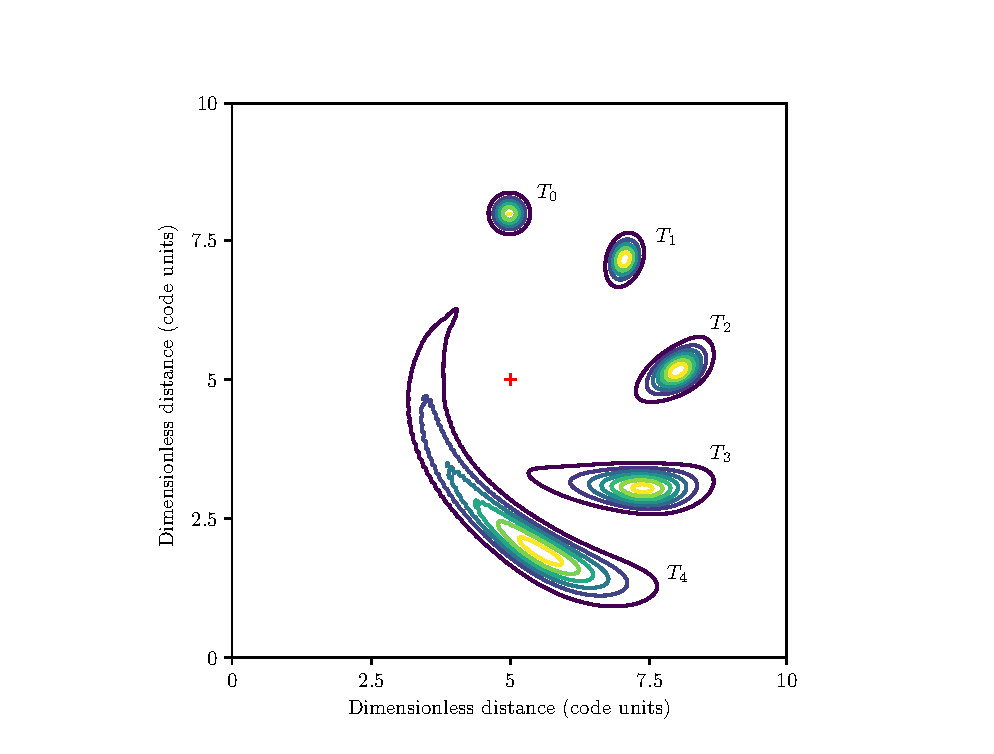
\includegraphics[width=1.\textwidth,trim=0 0 0 0,clip]{density_diagram1}
% \caption{Density profile of solitonic core at equally spaced times as it undergoes tidal disruption in a potential centred at the red cross.}\label{fig:density_diagram1}
% \end{figure}

% \begin{figure}[tbp]
% \centering 
% 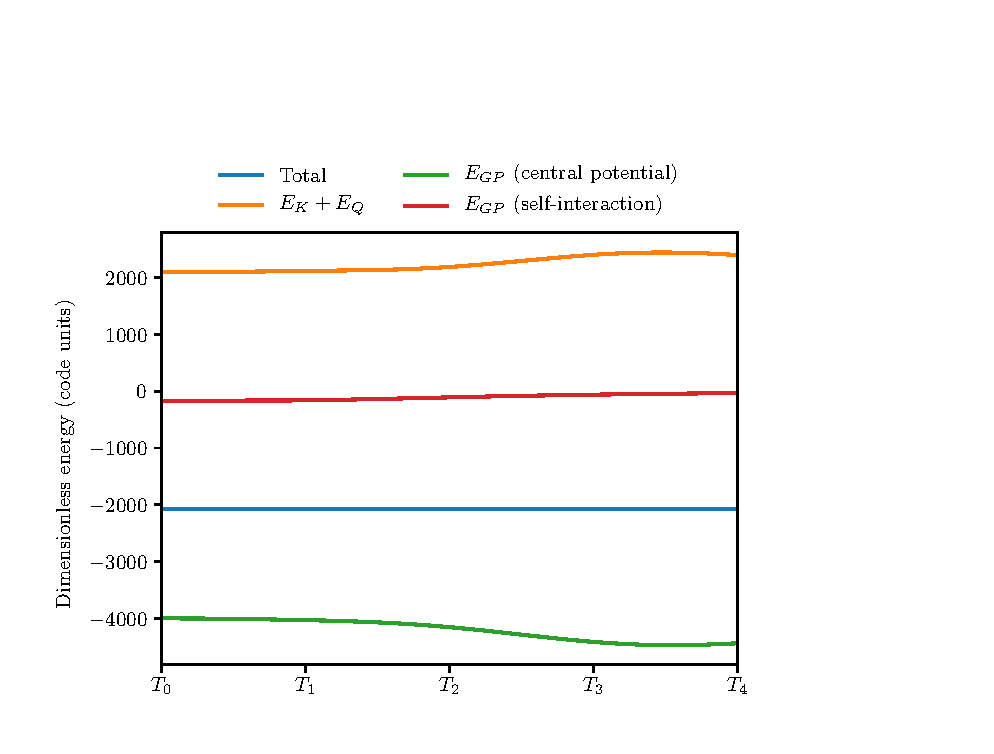
\includegraphics[width=1.\textwidth,trim=0 0 0 0,clip]{energy_diagram1}
% \caption{Evolution of the energy of the system illustrated in Figure \ref{fig:density_diagram1}. Times are indicated in correspondence with the snapshots of the density profile. }\label{fig:energy_diagram_1}
% \end{figure}

% \begin{figure}[tbp]
% \centering 
% 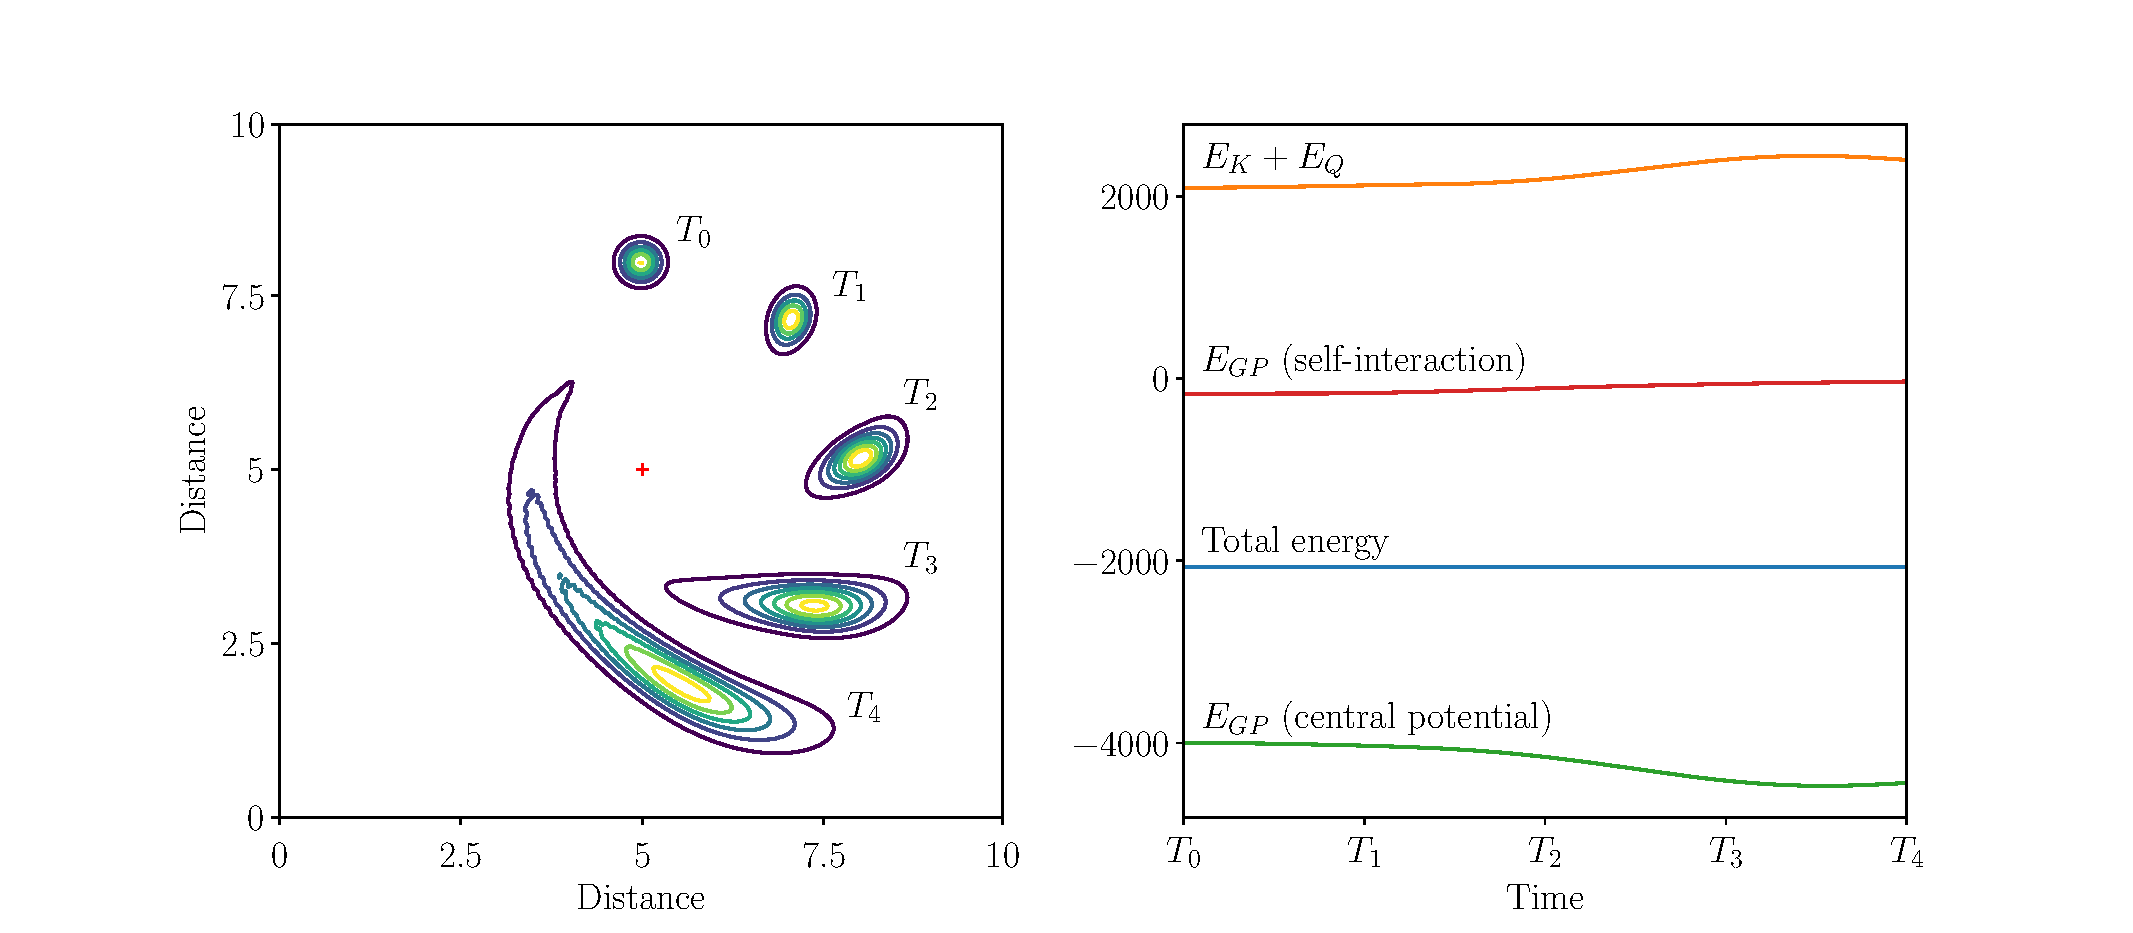
\includegraphics[width=1.1\textwidth,trim=2.5cm 0 0 1cm,clip]{combined_energy_and_density1}
% \caption{Left: Evolution of the density profile of a solitonic core at equally spaced times as it undergoes tidal disruption in a potential centred at the red cross. Right: Evolution of the energy of the system, where times are indicated in correspondence with the snapshots of the density profile. All quantities are in dimensionless code units.}\label{fig:combined_1}
% \end{figure}

% \begin{figure}[tbp]
% \centering 
% 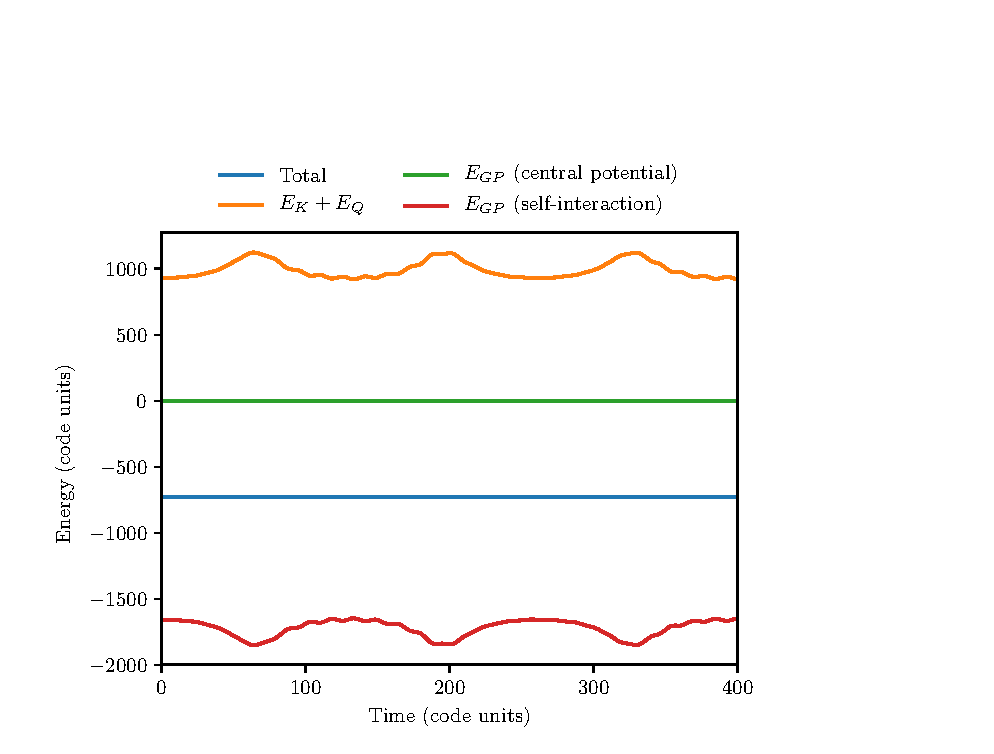
\includegraphics[width=1.\textwidth,trim=0 0 2cm 2cm,clip]{energy_diagram2}
% \caption{Evolution of the energy for a binary soliton system with each soliton in an elliptical orbit around the common centre of mass.}\label{fig:binary}
% \end{figure}


\begin{figure}
  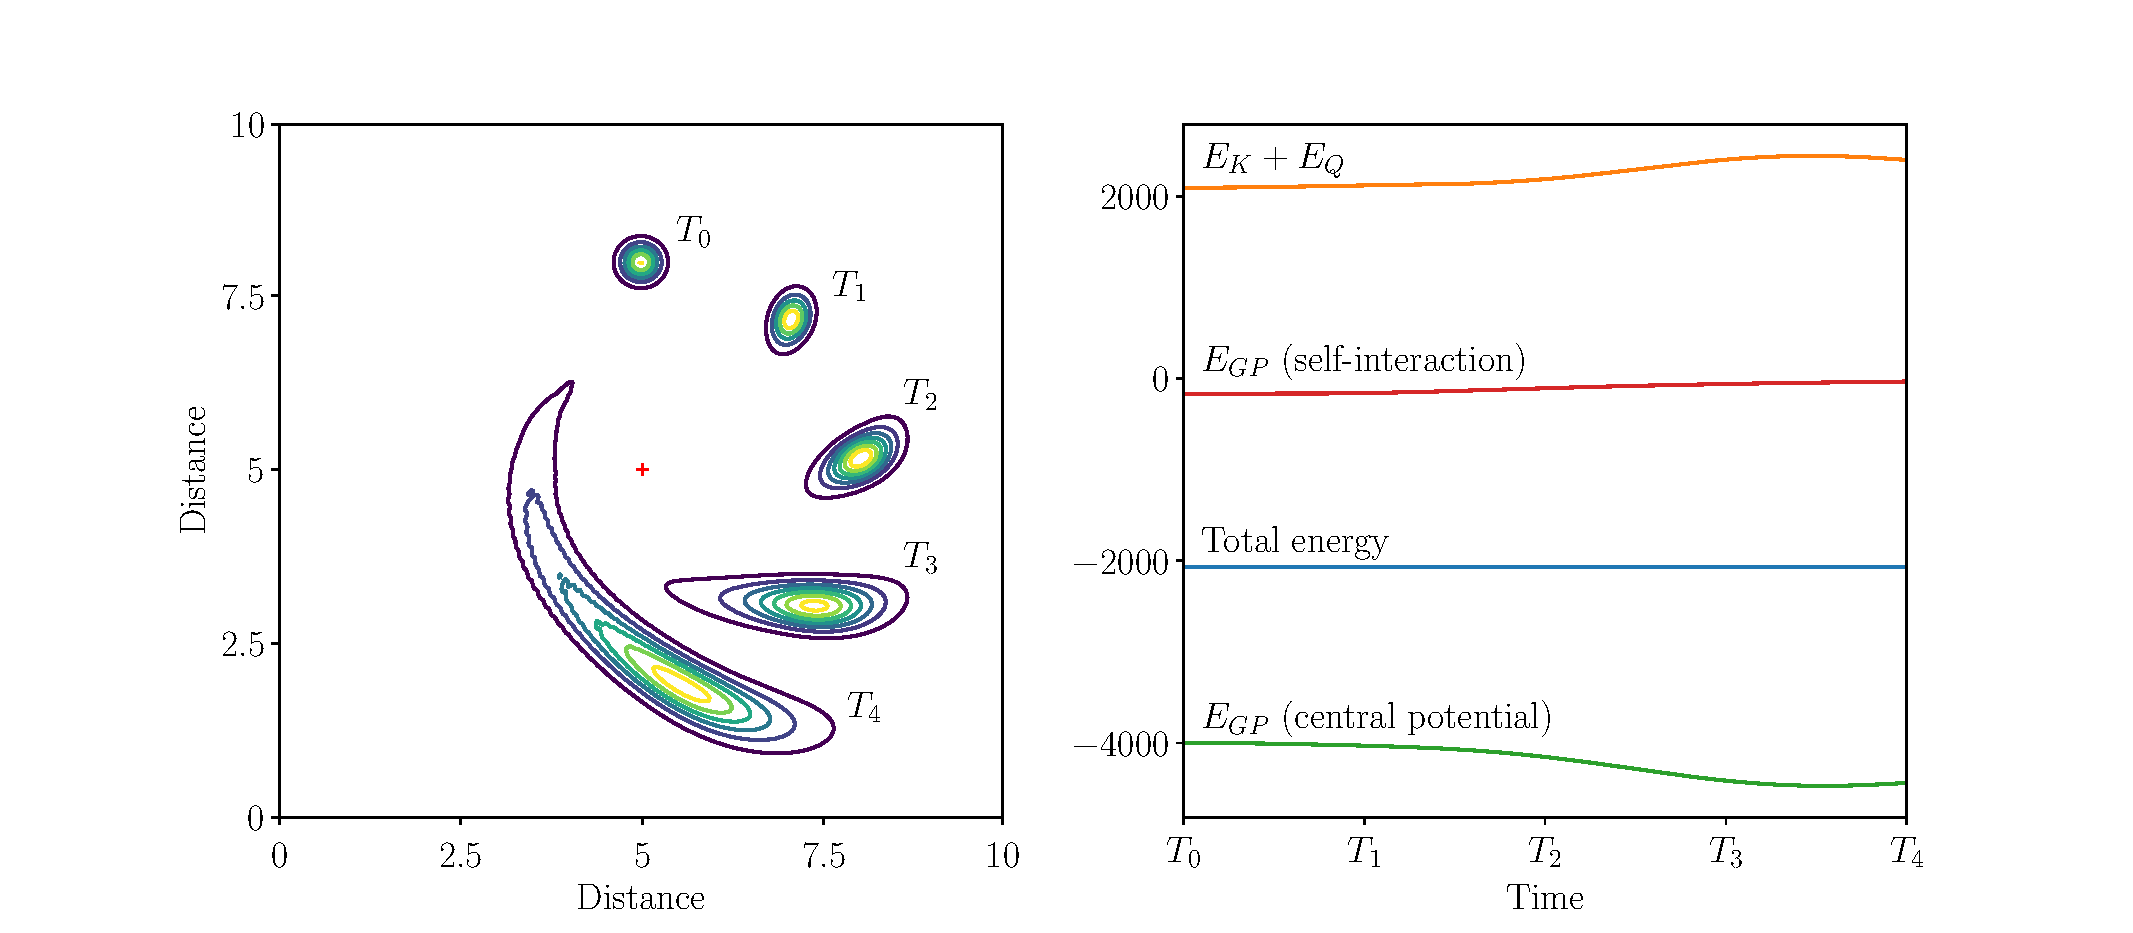
\includegraphics[width=1.1\textwidth,trim=2.5cm 0 0 1cm,clip]{combined_energy_and_density1}
  \caption{Left: Evolution of the density profile of a solitonic core at equally spaced times as it undergoes tidal disruption in a potential centred at the red cross. Right: Evolution of the energy of the system, where times are indicated in correspondence with the snapshots of the density profile. All quantities are in dimensionless code units.}
  \label{fig:combined_1}
\end{figure}

\begin{figure}
  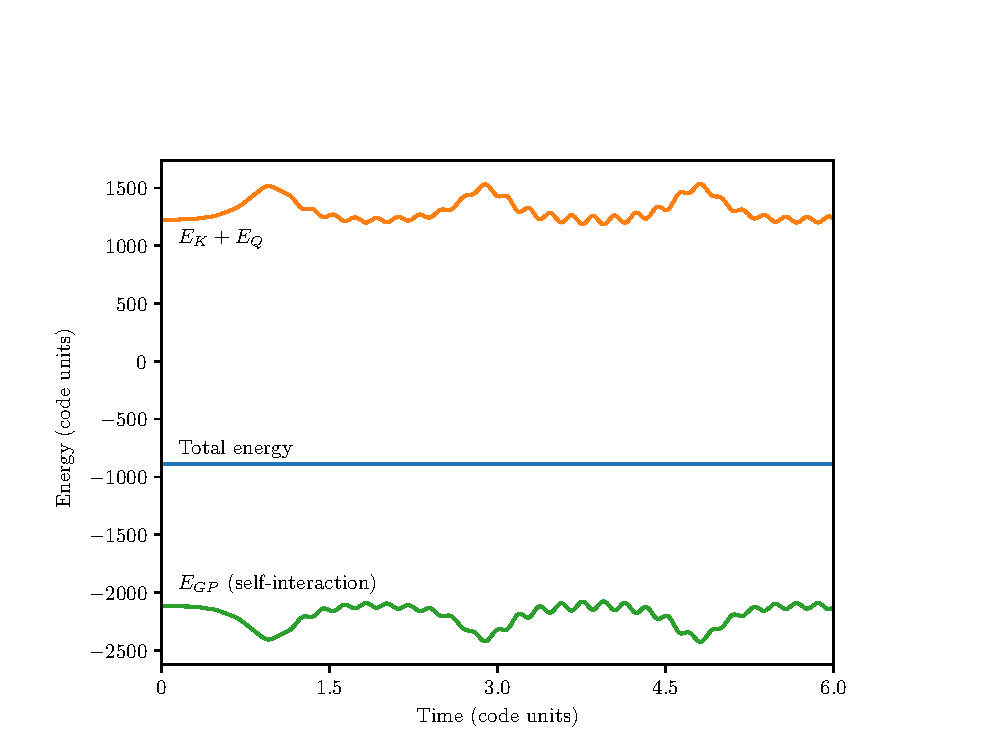
\includegraphics[width=0.9\textwidth,trim=0 0 2cm 2cm,clip]{egy_m=22.eps}
  \caption{Evolution of the energy for a binary soliton system with each soliton in an elliptical orbit around the common centre of mass.}
  \label{fig:binary}
\end{figure}





\section{Discussion and Outlook}

We have demonstrated that \PyUltraLight is an accurate tool for the study of the dynamics of ultralight dark matter governed by the Schr{\"o}dinger-Poisson system of equations. The code makes use of a pseudo-spectral symmetrised split-step Fourier methodology, in which all spatial derivatives are treated via explicit multiplication in the Fourier domain, thereby avoiding difficulties associated with finite-differencing methods. 

Energy conservation within \PyUltraLight is excellent, at sub-percent level for simulations run at $128^3$, and even better performance as resolution is increased. The code is able to reproduce complex phenomena resulting from the wave-like properties of ultralight dark matter as predicted by theoretical models, such as the interference patterns arising during high-velocity collisions of solitonic cores, and the effective forces observed in cases where the colliding cores are out of phase. These phenomena can be clearly observed at relatively low spatial resolution, obviating the need for high-performance computing infrastructure to study the fundamental behaviour of ULDM systems. This makes \PyUltraLight a useful tool for predicting the overall dynamics of a ULDM system in a computationally efficient manner prior to a rigorous examination using more advanced codes such as Nyx.

\PyUltraLight is Python-based, and as such is particularly simple to understand and use. The accompanying Jupyter notebook allows for the efficient adjustment of simulation parameters, and offers a useful browser interface for quick visualisation of simulation results. Despite being Python-based, the code makes use of low-level language resources, namely the FFTW libraries through the use of the Pythonic pyFFTW wrapper. 

While the current implementation of \PyUltraLight is already a useful tool for simulating dynamical ULDM systems, there remains scope for substantial improvement. In particular, it is anticipated that future releases may incorporate adaptive mesh refinement capabilities and variable timestep functionality. Additionally, while the current implementation utilises a spatial grid of fixed size and does not provide a means by which to incorporate baryonic density contributions, future releases are likely to allow for cosmic expansion and a means by which to incorporate simplified models of baryonic matter. Further adaptations of the code may also be implemented to allow for greater flexibility in the choice of ULDM model, incorporating possibilities such as explicit self-interaction. 





\appendix
\section{Download and Licensing}

\PyUltraLight has been made publicly available under a BSD licence. The full code repository, including supplementary files such as the code used to generate soliton profiles, is available on GitHub at https://github.com/erckendall/PyUltraLight. \PyUltraLight makes use of the pyFFTW pythonic wrapper around the FFTW C-based fast Fourier transform libraries. Both pyFFTW and FFTW are freely-available. \PyUltraLight has been successfully tested on both Mac OS and Linux operating systems, though not exhaustively. The current version of \PyUltraLight, as demonstrated in this work, is capable of reproducing many of the results of previous ULDM simulations, and we plan to extend its capabilities in future releases.  

\acknowledgments

TBW



% The bibliography will probably be heavily edited during typesetting.
% We'll parse it and, using the arxiv number or the journal data, will
% query inspire, trying to verify the data (this will probalby spot
% eventual typos) and retrive the document DOI and eventual errata.
% We however suggest to always provide author, title and journal data:
% in short all the informations that clearly identify a document.

%\section*{References}
\bibliographystyle{JHEP}
\bibliography{refs} 


%\begin{thebibliography}{99}

%\bibitem{a}
%Author, \emph{Title}, \emph{J. Abbrev.} {\bf vol} (year) pg.

%\bibitem{b}
%Author, \emph{Title},
%arxiv:1234.5678.

%\bibitem{c}
%Author, \emph{Title},
%Publisher (year).

% Please avoid comments such as "For a review'', "For some examples",
% "and references therein" or move them in the text. In general,
% please leave only references in the bibliography and move all
% accessory text in footnotes.

% Also, please have only one work for each \bibitem.

%\end{thebibliography}

\end{document}
